\documentclass[a4paper]{article}

\usepackage[a4paper,margin=2cm]{geometry}
\usepackage{amsmath}
\usepackage{graphicx}
\usepackage[table]{xcolor}
\usepackage{tikz}
\usepackage{minted}
\usepackage[clock]{ifsym}
\usepackage{subcaption} % subfigures
\usepackage{hyperref} % links in table of contents
\usepackage[strings]{underscore}

\usetikzlibrary{calc,positioning,shapes,arrows.meta,decorations.pathreplacing}
\graphicspath{ {./graphics/} }

\hypersetup{
	colorlinks,
	citecolor=black,
	filecolor=black,
	linkcolor=black,
	urlcolor=black
}
\numberwithin{figure}{section}
\numberwithin{table}{section}
\renewcommand{\arraystretch}{1.5}

\newcommand{\mi}{\mintinline}
\newcommand{\NA}{---}

\title{CS2022 - Project 2}
\date{2019-04-14}
\author{\url{https://git.nul.ie/dev/cs2022}\\\url{https://github.com/devplayer0/cs2022}\\Jack O'Sullivan\\\href{mailto:osullj19@tcd.ie}{osullj19@tcd.ie}\\17331147}

\begin{document}
\maketitle
\tableofcontents
\pagenumbering{gobble}

\newpage
\pagenumbering{arabic}
\section{Introduction}
The goal of this assignment was to complete a functional microprogrammed processor, implementing a number of intructions.

\section{Testbench results}
This section details results of the testbenches for the components created in project 2.

\subsection{\mi{c}{memory}}
\begin{figure}[h!]
	\centering
	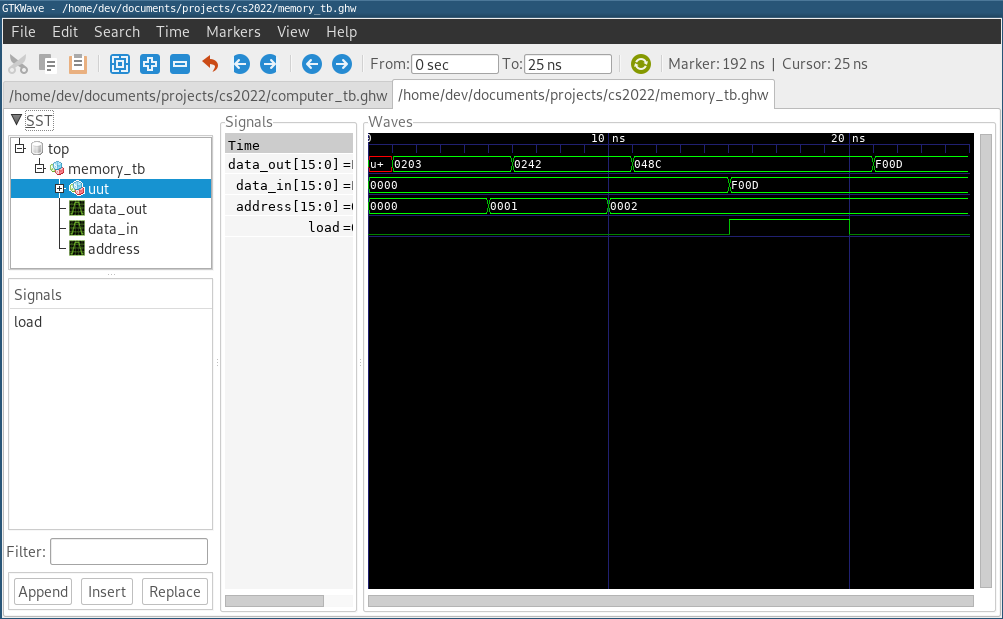
\includegraphics[width=\textwidth]{memory_tb}
	\caption{\mi{c}{memory} testbench results}
	\label{fig:memory}
\end{figure}

Figure~\ref{fig:memory} shows the simulation results of the 512x 16-bit word main memory.
\begin{itemize}
	\item After a short delay, setting the input address to \mi{c}{0} produces \mi{c}{0x203} (the first instruction in memory) at \mi{c}{data_out}.
	\item Increasing the address shows the following instructions.
	\item Setting \mi{c}{data_in} and the load signal to high shows that the data at \mi{c}{0x2} is overwritten.
\end{itemize}

\end{document}
# vim: nofoldenable
